\documentclass{article}
\usepackage[utf8]{inputenc}
\usepackage{listings}
\usepackage{xcolor}
\usepackage{graphicx}

% Definir colores para el resaltado de sintaxis
\definecolor{codegreen}{rgb}{0,0.6,0}
\definecolor{codegray}{rgb}{0.5,0.5,0.5}
\definecolor{codepurple}{rgb}{0.58,0,0.82}
\definecolor{backcolour}{rgb}{0.95,0.95,0.92}

% Configuración para el código JavaScript
\lstdefinestyle{mystyle}{
    backgroundcolor=\color{backcolour},
    commentstyle=\color{codegreen},
    keywordstyle=\color{magenta},
    numberstyle=\tiny\color{codegray},
    stringstyle=\color{codepurple},
    basicstyle=\footnotesize,
    breakatwhitespace=false,
    breaklines=true,
    captionpos=b,
    keepspaces=true,
    numbers=left,
    numbersep=5pt,
    showspaces=false,
    showstringspaces=false,
    showtabs=false,
    tabsize=2
}

% Configuración para el lenguaje JavaScript
\lstset{style=mystyle, language=JavaScript}

\title{Profundidad de Herencia en el Desarrollo de Software}
\author{Paul Wenceslao Condori Garcia}


\begin{document}

\maketitle

\section{Profundidad de Herencia} 

La herencia es uno de los elementos clave que hacen poderosa la programación orientada a objetos \cite{meyer1997object}. Muchos problemas de diseño pueden resolverse con elegancia utilizando la herencia y el polimorfismo, y los diseños resultantes suelen ser más sencillos, claros y flexibles de lo que podrían haberse conseguido de otro modo  \cite{gamma1995design}. Pero también es obvio que la construcción de herencia puede introducir complejidad adicional si se utiliza de forma inadecuada.\cite{Prechelt2003inheritance depth}

La profundidad de herencia es una métrica utilizada en la ingeniería de software para medir la jerarquía de clases en un sistema orientado a objetos. Esta métrica proporciona información sobre la complejidad y la estructura del diseño del software, y puede afectar varios aspectos del desarrollo y mantenimiento del sistema.\cite{Fenton1994SoftwareMetrics}
\begin{figure}
  \centering
    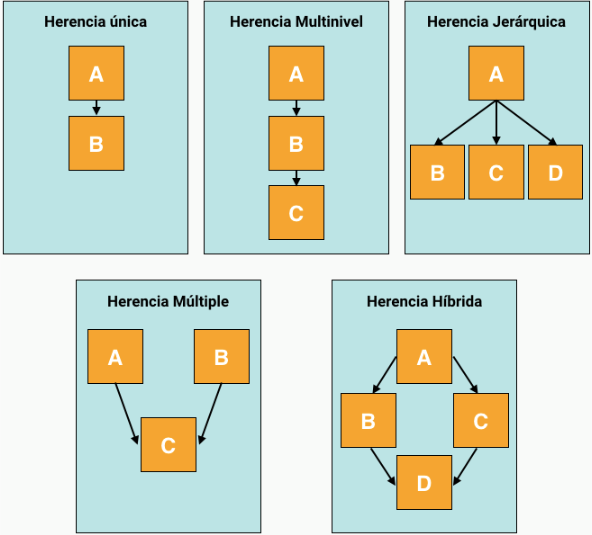
\includegraphics{hp1.png}
\end{figure}
\section{Definición y Tipos}

La profundidad de herencia se refiere al número máximo de niveles en la jerarquía de clases dentro de un sistema de software. Existen dos tipos principales de profundidad de herencia:
\begin{itemize}
    \item Profundidad Máxima de Herencia: Es el número máximo de niveles en la jerarquía de clases dentro de un sistema.
    \item Profundidad Promedio de Herencia: Es el promedio de la profundidad de herencia para todas las clases en el sistema.
\end{itemize}

\section{Aplicaciones y Limitaciones}

La profundidad de herencia se utiliza para evaluar la complejidad del diseño del software y puede tener implicaciones en la mantenibilidad, la comprensión del código y la reutilización de software. Una profundidad de herencia excesiva puede hacer que el sistema sea difícil de entender y mantener, aumentando la complejidad y el riesgo de errores.

\subsection{Ejemplo de Código en JavaScript para Profundidad de Herencia}

\begin{lstlisting}
// Definición de clases en una jerarquía de herencia
class Animal {
  constructor() {
    this.type = 'Animal';
  }
}
class Mamifero extends Animal {
  constructor() {
    super();
    this.category = 'Mamífero';
  }
}
class Perro extends Mamifero {
  constructor() {
    super();
    this.name = 'Perro';
  }
}
// Función para calcular la profundidad de herencia
function calcularProfundidadHerencia(clase) {
  let profundidad = 0;
  let prototipo = Object.getPrototypeOf(clase);
  while (prototipo !== null) {
    profundidad++;
    prototipo = Object.getPrototypeOf(prototipo);
  }
  return profundidad;
}
// Ejemplo de uso de la función
console.log('Profundidad de herencia de la clase Perro:', calcularProfundidadHerencia(Perro)); // Resultado esperado: 2 (Perro <- Mamifero <- Animal)
\end{lstlisting}

Sin embargo, la profundidad de herencia también tiene limitaciones. No siempre es indicativa de la calidad del diseño del software, ya que una profundidad de herencia baja no garantiza un diseño óptimo y una profundidad de herencia alta no siempre indica un diseño deficiente. Además, puede haber casos donde una profundidad de herencia alta sea necesaria para modelar adecuadamente la complejidad del dominio del problema. además, las pruebas empíricas sólidas sobre los efectos de la herencia son limitadas. El mecanismo de herencia no ha sido plenamente aceptado por la comunidad empírica.
\cite{Cartwright1998empirical_inheritance}

\section{Conclusiones}
La profundidad de herencia es una métrica importante en el diseño de software orientado a objetos, ya que proporciona información sobre la complejidad y la estructura del sistema. Al comprender y analizar la profundidad de herencia, los equipos de desarrollo pueden tomar decisiones informadas sobre el diseño y la arquitectura del software.

\section{Referencias}

\begin{thebibliography}{9}
\bibitem{meyer1997object} 
Meyer, B. (1997). Object-oriented software construction. Prentice Hall PTR.
\bibitem{gamma1995design} 
Gamma, E., Helm, R., Johnson, R., \& Vlissides, J. (1995). Design patterns: elements of reusable object-oriented software. Pearson Education.
\bibitem{Fenton1994SoftwareMetrics}
Fenton, N. E., Pfleeger, S. L. (1994). Software Metrics: A Rigorous and Practical Approach. PWS Publishing Co.
\bibitem{Prechelt2003inheritance_depth}
Prechelt, L., Unger, B., Philippsen, M., and Tichy, W. (2003). A controlled experiment on inheritance depth as a cost factor for code maintenance. Journal of Systems and Software, 65(2), 115-126.
\bibitem{Cartwright1998empirical_inheritance}
Cartwright, M. (1998). An empirical view of inheritance. Information and Software Technology, 40(14), 795-799.
\end{thebibliography}
\end{document}
